% !TeX root = ../Avances.tex


\section{Conclusiones y trabajo a futuro}

\begin{frame}{Conclusiones}{Para una AuNP de 12.5 m, de radio parcialmente embebida entre un sustrato plano y una matriz}

  \begin{center}
  	\begin{tikzpicture}[node distance=1em and 1em,font=\small]

        \path (0,0) node [flowbox] (inc) {
        \fbtitle{Incrustación}\vphantom{yÖ}
	    \nodepart{two}
         \begin{minipage}{.28\textwidth}
         A lo más un octavo del  volumen en
         \begin{itemize}
			\item Sustrato $\to$ AuNP soportada
			\item Matriz $\to$ AuNP totalmente embebida
         \end{itemize}
         \end{minipage}
        };


	\node[flowbox,left=of inc] (trans) {
        \fbtitle{Transición}\vphantom{yÖ}
    \nodepart{two}
        \begin{minipage}{.28\textwidth}\begin{itemize}
			\item  Contribución mayormente dipolar
  	\item Transición \textit{suave} entre los dos casos límites de Mie
         \end{itemize}\end{minipage}
    };

    \node[flowbox,right=of inc] (pol) {
        \fbtitle{Iluminación}\vphantom{yÖ}
    \nodepart{two}
        \begin{minipage}{.28\textwidth}
        Resonancia y la distribución espacial del campo eléctrico
        \begin{itemize}
			\item  Pol. $s$:  no dependen de el ángulo de incidencia.
			\item Pol. $p$: sí dependen de el ángulo de incidencia.
         \end{itemize}
         $\theta_i \approx \theta_c$: Máximización de la extinción
		\end{minipage}
    };

    \node[below = of inc]{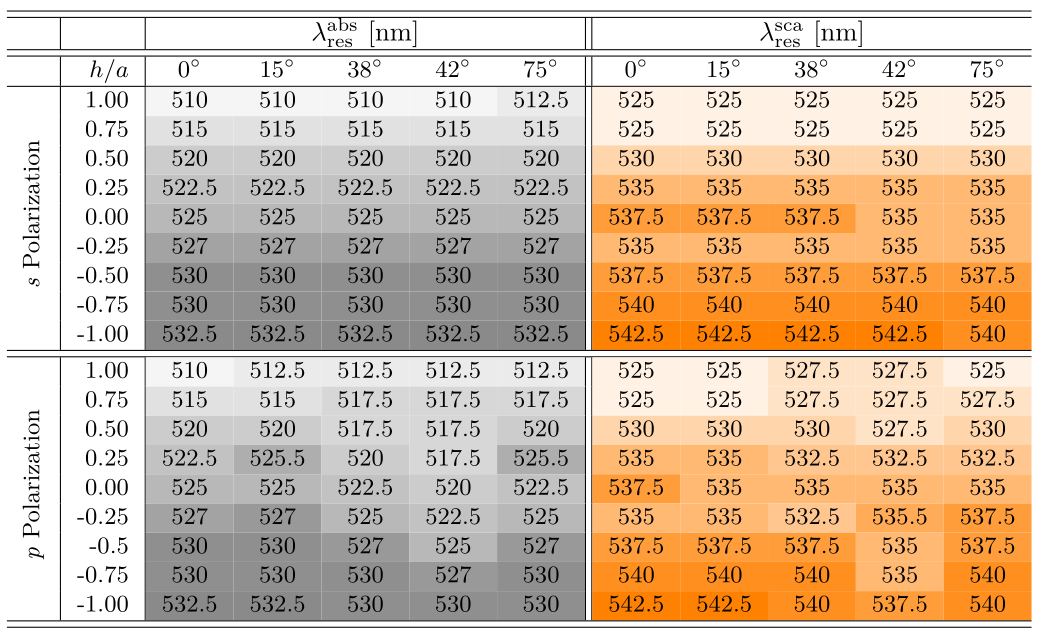
\includegraphics[scale  = .15]{Trans.png}};
    \node[below = of trans]{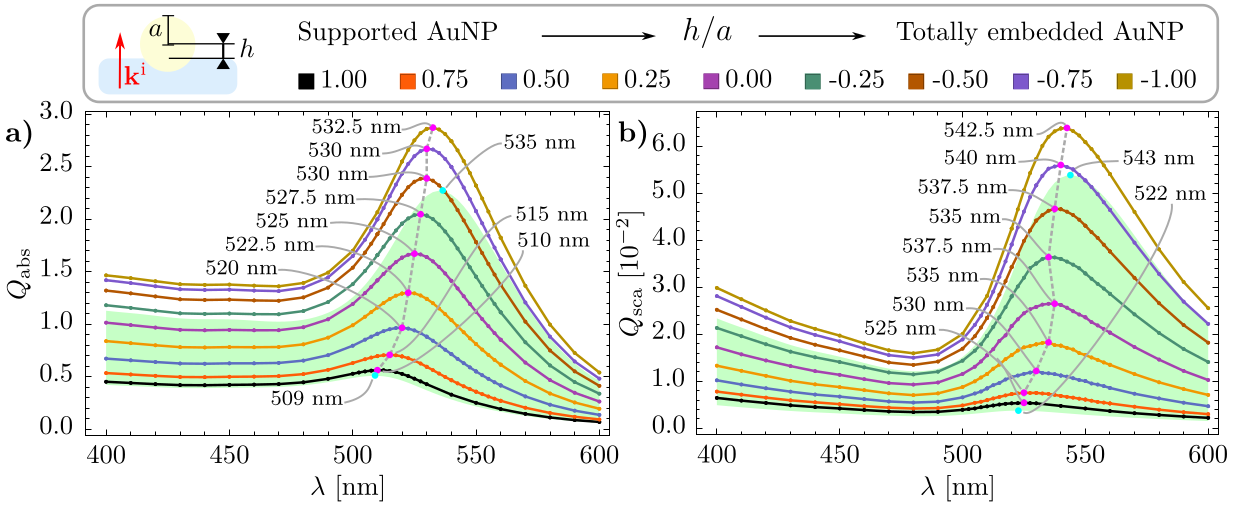
\includegraphics[scale  = .15]{Dip-Mie.png}};
    \node[below = of pol]{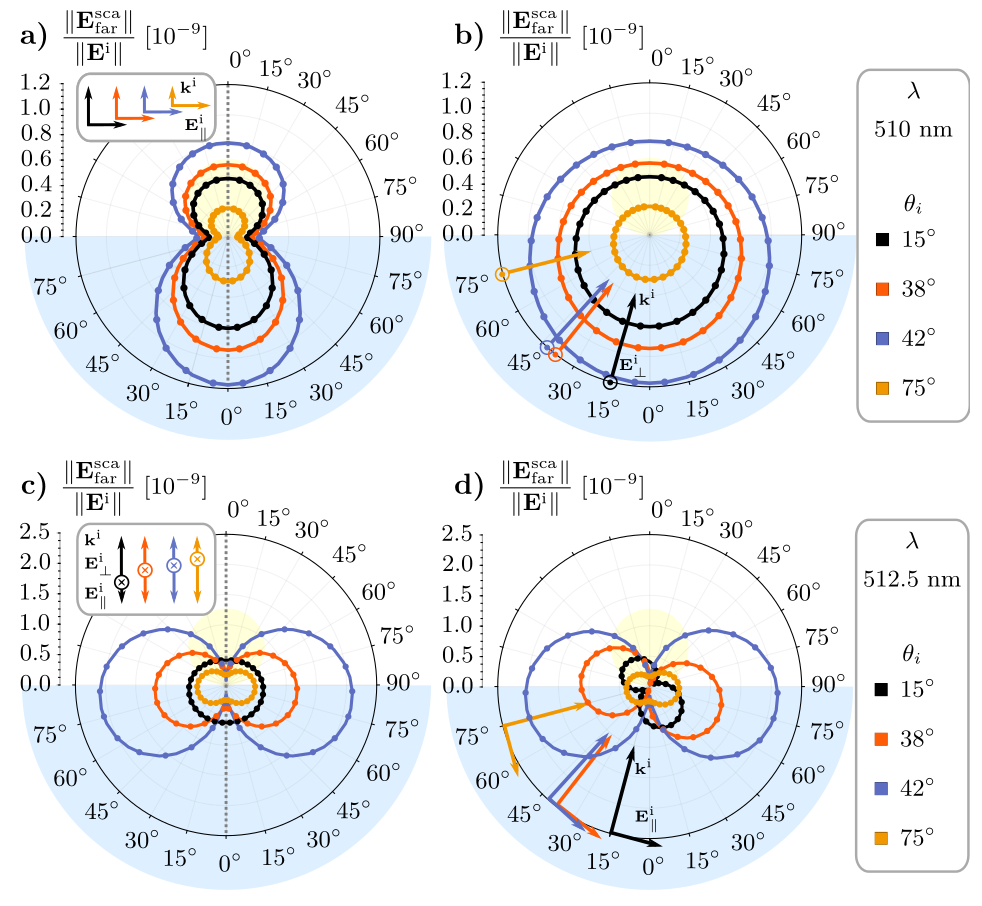
\includegraphics[scale  = .15]{Distribucion.png}};
  \end{tikzpicture}
  \end{center}

\end{frame}



\begin{frame}{Trabajo a futuro}{Para una NP parcialmente embebida entre un sustrato plano y una matriz}

  \begin{center}
  	\begin{tikzpicture}[node distance=1em and 1em]

        \path (0,0) node [flowbox] (meta) {
        \fbtitle{Propiedades ópticas del meta-átomo (Cálculos numéricos)}\vphantom{yÖ}
	    \nodepart{two}
         \begin{minipage}{.85\textwidth}\small
         Determinar secciones transversales como función de la longitud de onda $\lambda$ y polarización de la onda plana que ilumina el sistema, del ángulo de incidencia $\theta_i$ y el grado de incrustación $h/a$ del meta-átomo.
         \end{minipage}
        };

    \path (-3.75,-3) node [flowbox] (eff) {
        \fbtitle{Homogenización + Medio efectivo}\vphantom{yÖ}
	    \nodepart{two}
         \begin{minipage}{.45\textwidth}\small
         Proponer un modelo semi-analítico para la respuesta óptica de una monocapa parcialmente incrustrada:\\

         \begin{itemize}
			\item Homogenización tipo Brüggemman$^1$ del índice de refracción efectivo que envuelve a las NPs.
			\item Empleo de teorías como el Modelo Dipolar$^2$, Teoría de Islas Delgadas$^3$ para la respuesta del sistema monocapa.
         \end{itemize}
         \end{minipage}
        };

    \path (3.75,-3.35) node [flowbox] (exp) {
        \fbtitle{Medición del incrustamiento promedio}\vphantom{yÖ}
	    \nodepart{two}
         \begin{minipage}{.45\textwidth}\small
         Propuesta de un esquema de medición para medir el incrustamiento promedio de la monocapa:\\

         \begin{itemize}
			\item Medición de la $\lambda_{\text{res}}$ para al menos dos valores de $\theta_i>\theta_c$ en ambas polarizaciones.
			\item Comparar el corrimiento de $\lambda_{\text{res}}$ relativo entre ambas polarizaciones.
			\item Con base en las propiedades de un meta-átomo determinar a qué valores de $h/a$ corresponden las mediciones anteriores.
         \end{itemize}
         \end{minipage}
        };

    \draw[- latex, thick] (meta.south) -- (eff.north);
    \draw[- latex, thick] (meta.south) -- (exp.north);
    \end{tikzpicture}
    \end{center}

\noindent\rule{.25\textwidth}{0.4pt}\\
\fontsize{4}{5} \selectfont
	$^1$ \fullcite{sihvola_electromagnetic_2008}\\
	$^2$ \fullcite{barrera1991optical}\\
	$^3$ \fullcite{bedeaux_optical_2004}
\end{frame}

